\setcounter{page}{1}
\section*{Zielsetzung}
Im Versuch 601 soll die Quantelung der Energieniveaus von Queksilber-Atomen beobachtet werden.
Hierzu wird der nach James Franck und Gustav Hertz benannte Aufbau verwendet, der im Wesentlichen
den Energieverlust beschleunigter Elektronen beim elastischen Stoß mit Quecksilberatomen ausnutzt.

\section{Theorie}
Der prinzipielle Aufbau des Franck-Hertz-Versuches ist in Abbildung \ref{fig: schema_aufbau} dargestellt. Innerhalb
eines mit Quecksilberdampf gefüllten Glaskolbens befinden sich ein Glühdraht, eine Beschleunigungselektrode und
eine Auffängerelektrode. Durch eine konstante Gleichspannung am Glühdraht wird dieser bis zum Glühen
erhitzt, was zur Elektronenemession führt (Glühelektrischer Effekt).
\begin{figure}
  \centering
  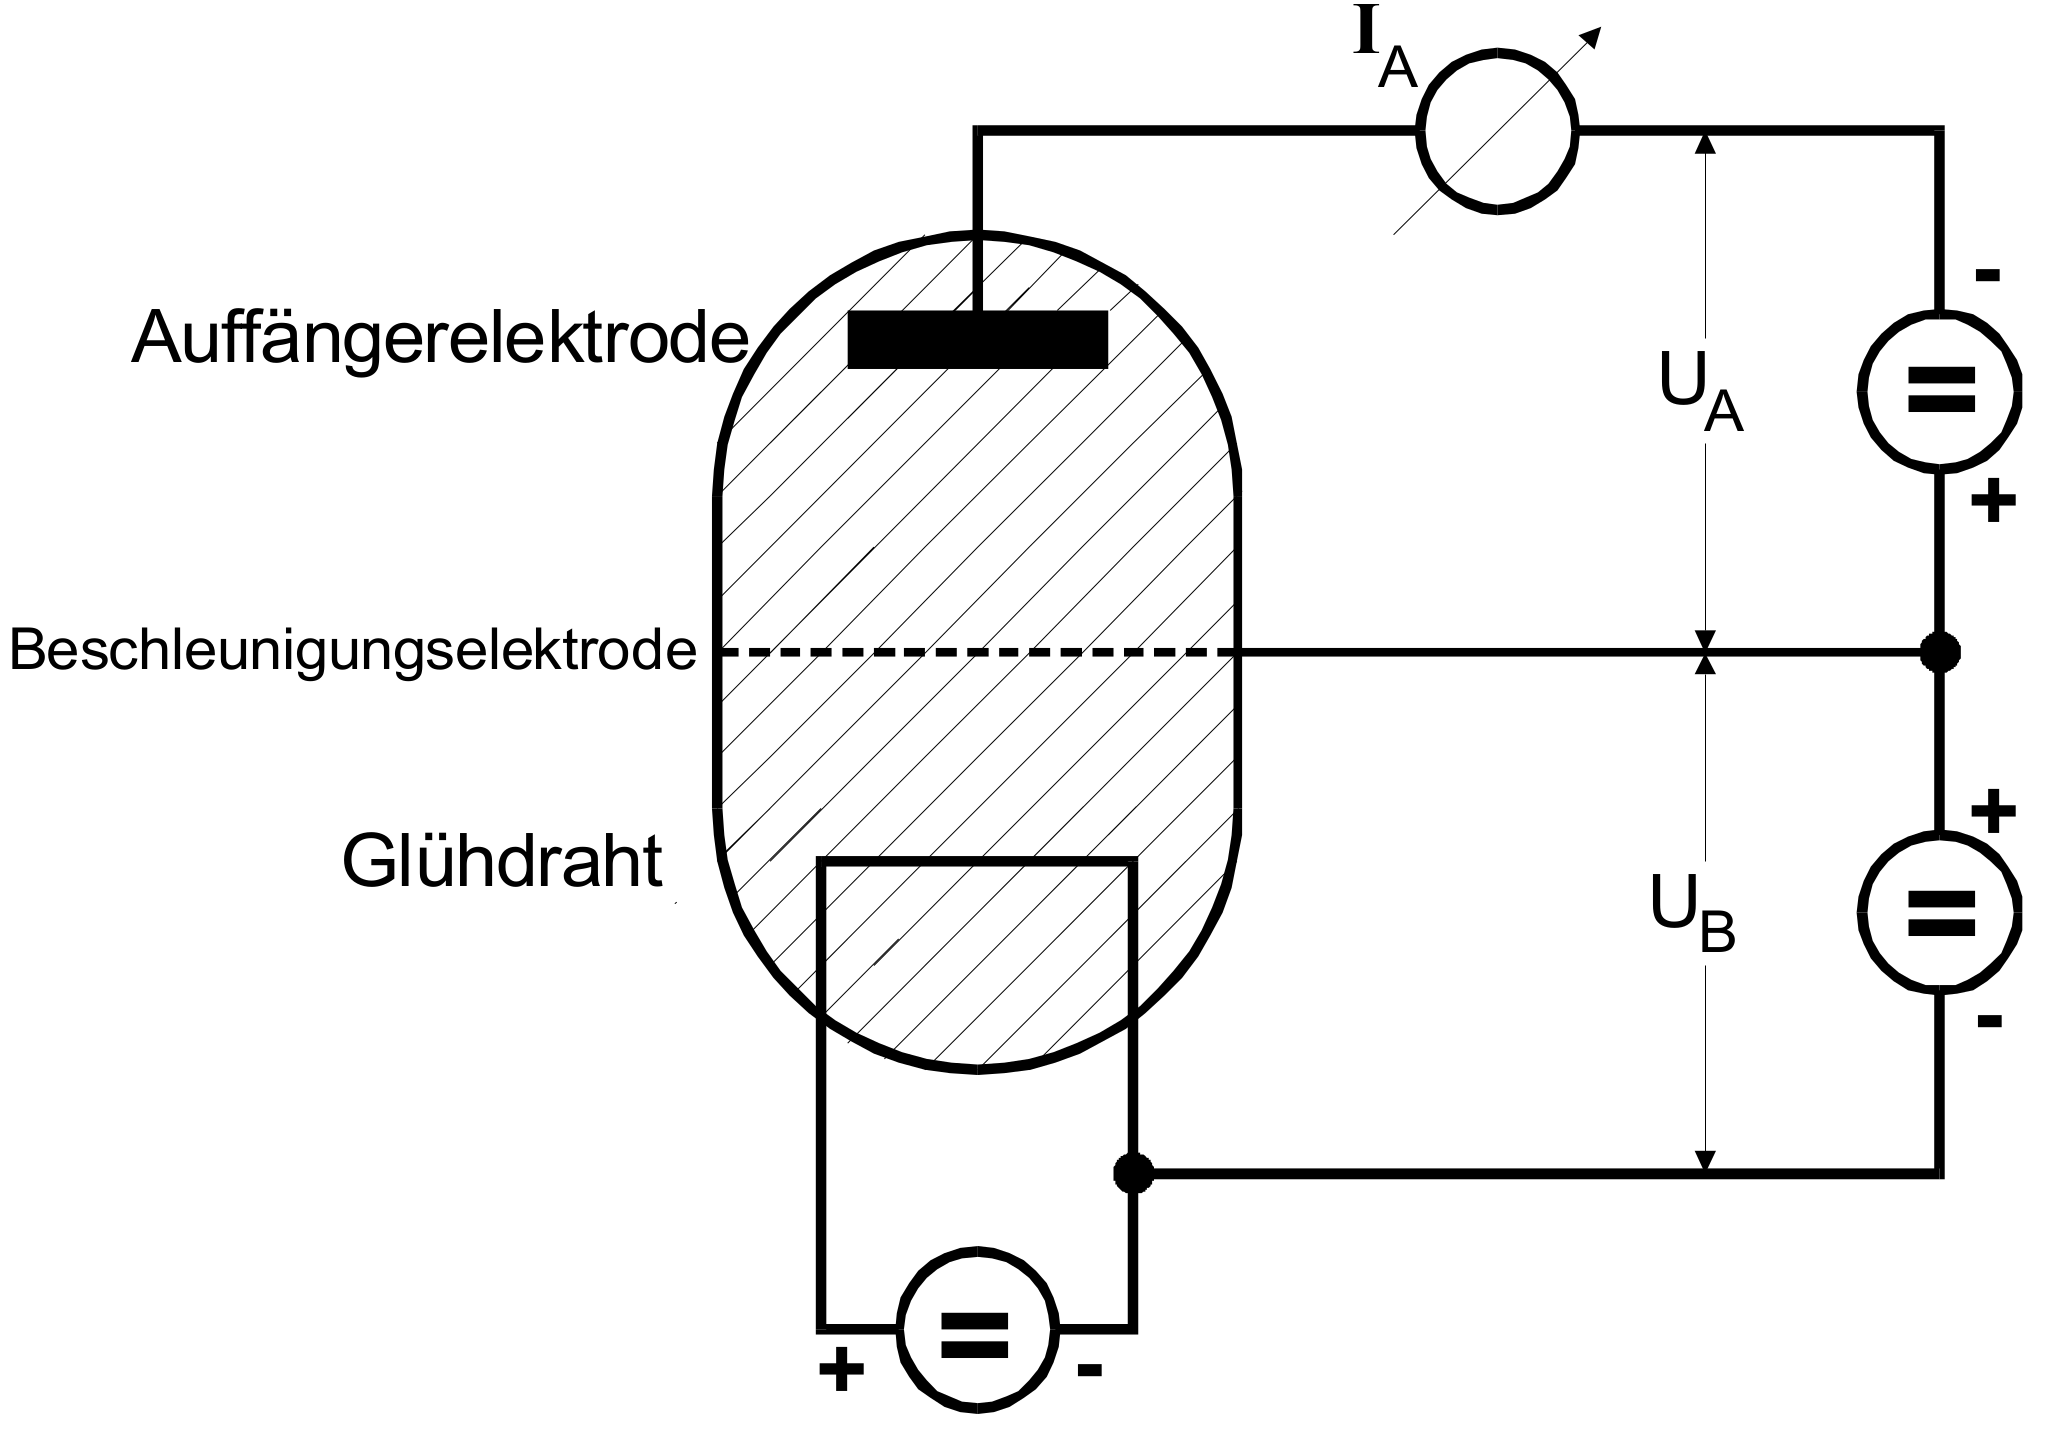
\includegraphics[width = 0.5\textwidth]{pics/schema_aufbau.png}
  \caption{Schematische Darstellung des Franck-Hertz-Aufbaus \cite{anleitung601}.}
  \label{fig: schema_aufbau}
\end{figure}
Die nun freien Elektronen werden durch die Spannung $U\ua{B}$ in Richtung der Beschleunigungselektrode
beschleunigt. Hinter der gitterförmigen Beschleuinigungselektrode ist eine Gegenspannung $U\ua{A}$ angelegt, die zum Abbremsen %gitterförmig
der Elektronen führt. Es gelangen nur solche Elektronen zur Auffängerelektrode, für deren kinetische Energie $E\ua{kin}$
gilt
\begin{equation}
 \label{eq: ungl_E_kin}
  E\ua{kin} = \frac{1}{2}m\ua{e}v^2 \geq \mathup{e}\ua{0}U\ua{A}.
\end{equation}
Der an der Auffängerelektrode messbare Strom $I\ua{A}$ stellt somit ein qualitatives Maß für die Anzahl der
Elektronen dar, deren Energien die Ungleichung \eqref{eq: ungl_E_kin} erfüllen.\\
Nun finden elastische und inelastische Stöße zwischen den Elektronen und den \ce{Hg}-Atomen statt. Gemäß %Nun kommt klingt nicht so schön
den aus der klassischen Mechanik bekannten Zusammenhängen für den elastischen Stoß ist die Energieabgabe
des Elektrons in diesem Fall maximal
\begin{equation}
  \Delta E = \frac{4 m\ua{e}}{m\ua{Hg}} \approx \num{e-5}.
\end{equation}
Dieser Effekt ist für den Energieverlust somit vernachlässigbar. Elastische Stöße zwischen Elektron und
\ce{Hg}-Atom finden immer dann statt, wenn die Energie $E\ua{kin}$ mindestens der Energiedifferenz $E\ua{1} - E\ua{0}$
zwischen dem ersten angeregten und Grundzustand des \ce{Hg} Atoms entspricht. Der Prozess lässt sich wie folgt darstellen
\begin{equation}
  e^{-} + \ce{Hg} \longrightarrow \ce{Hg}^{*} + e^{-} + \Delta E\ua{kin}.
\end{equation}
Hierbei entspricht $\Delta E\ua{kin}$ dem Energiverlust des Elektrons und $\ce{Hg}^*$ dem angeregten Zustand des
\ce{Hg}-Atoms. Dieses kehrt nach einem kurzen Zeitabstand unter Aussendung eines Lichtquants der Energie bzw. Wellenlänge
\begin{equation}
  \map{h}\nu = E\ua{1} - E\ua{0} \quad \Rightarrow \quad \lambda = \frac{\map{h} c}{E\ua{1} - E\ua{0}}
  \label{eq: wellenlänge}
\end{equation}
in seinen Grundzustand zurück. Unter steigender Beschleunigungsspannung $U\ua{B}$ wird also immer dann ein
abrupter Abfall des Anodenstroms $I\ua{A}$ erwartet, wenn die Energie der Elektronen nach dem $n$-ten Stoß gerade
ausreicht um zum $(n+1)$ten mal erneut ein \ce{Hg}-Atom anzuregen. Bei weiterer Erhöhung der Beschleunigungsspannung
steigt der Strom erneut bis zu einem Maximum an, nachdem $U\ua{B}$ mindestens um $U\ua{A}$ erhöht wurde.
Der theoretische Verlauf des Zusammenhangs zwischen
$U\ua{B}$ und $I\ua{A}$ ist in Abbildung \ref{fig: theo_verlauf} wiedergegeben.
\begin{figure}
  \centering
  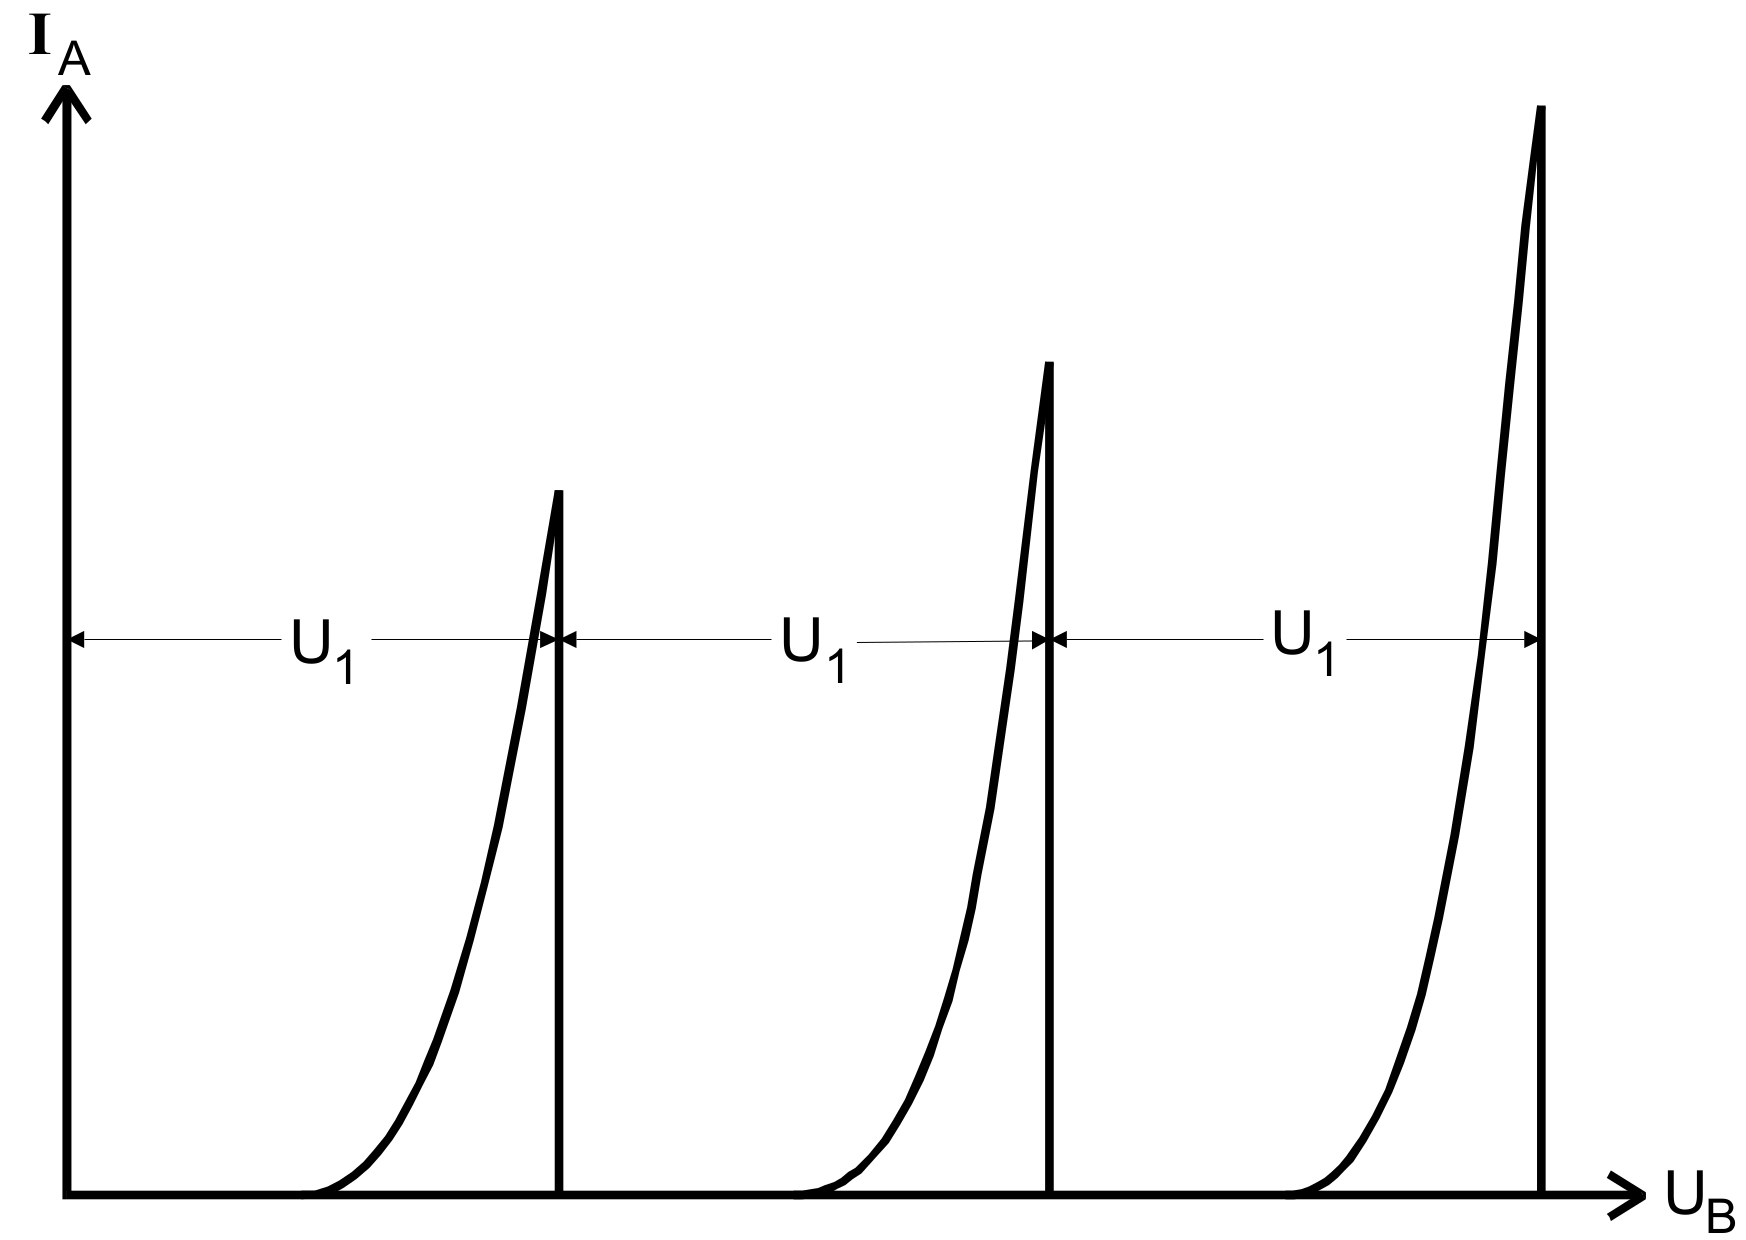
\includegraphics[width = 0.5\textwidth]{pics/theo_verlauf.png}
  \caption{Idealisierter Zusammenhang zwischen Beschleunigungsspannung $U\ua{B}$ und Anodenstrom $I\ua{A}$ \cite{anleitung601}.}
  \label{fig: theo_verlauf}
\end{figure}
Die zur Spannungsdifferenz $U\ua{1}$ gehörige
Energie $\mathup{e}\ua{0}U\ua{1}$ entspricht genau der Energiedifferenz $E\ua{1} - E\ua{0}$:
\begin{equation}
  \label{eq: anregungsenergie}
  E\ua{ex} = \mathup{e}\ua{0}U\ua{1}.
\end{equation}
Der theoretische
Verlauf \ref{fig: theo_verlauf} wird in der realen Messung durch verschiedene Einflüsse beeinträchtigt. \\
Um einen möglichst hohe Emissionsrate am Glühdrah zu erzielen, wird dieser aus Materialien mit möglichst geringer Austrittsarbeit $\varphi\ua{G}$ %Glühdraht
hergestellt (etwa Wolfram). An der Beschleunigungselektrode ist der glühelektrische Effekt unbedingt zu vermeiden, hier wird also
ein Material mit hoher Austrittsarbeit $\varphi\ua{B}$ verwendet. Zwischen Draht und Elektrode besteht das tatsächliche
Potential $V\ua{eff}$
\begin{equation}
  V\ua{eff} = \mathup{e}\ua{0} U\ua{B} - \left(\varphi\ua{B} - \varphi\ua{G}  \right).
\end{equation}
Die reale Franck-Hertz Kurve ist daher wie folgt verschoben
\begin{equation}
  \label{eq: effektivspannung}
  U\ua{B, eff} = U\ua{B} - \frac{1}{\mathup{e}\ua{0}}\left(\varphi\ua{B} - \varphi\ua{G}  \right) := U\ua{B}  - K.
\end{equation}
Darüber hinaus spielt der Gasdruck $p$ im Glaskolben eine wesentliche Rolle. Dieser hängt gemäß der Dampfdruck-Kurve
\begin{equation}
  \label{eq: dampfdruck}
  p(T) = \num{5.5e7}\exp \left( -\frac{6876}{T} \right) \quad \left\{[p] = \si{\milli\bar}, \, [T] = \si{\kelvin}\right\} % \qquad, und ich würde {} weglasssen
\end{equation}
mit der Umgebungstemepratur $T$ zusammen. Damit inelastische Stöße signifikant auftreten können muss die mittlere
freie Weglänge $\ov{w}$ im Gas
\begin{equation}
  \label{eq: weglaenge}
  \ov{w} = 0.0029 \frac{1}{p} \quad \left\{[\ov{w}] = \si{\centi\meter}, \, [p] = \si{\milli\bar} \right\}
\end{equation}
klein im Vergleich zum Abstand $a$ zwischen Draht und Beschleunigungselektrode sein (etwa um Faktor $1000$ bis $4000$). \\
Weiter genügen die Energien der Elektronen im Draht einer statistischen Verteilung. Daher finden die ineleastischen
Stöße nicht wie in \ref{fig: theo_verlauf} unter diskreten Spannungen $U\ua{B}$ statt. Der Anodenstrom fällt nicht abrupt
auf null sondern nähert sich stetig einem Minimum, wenn das Maximum der Energieverteilung einem Vielfachen der Energiedifferenz
zwischen Grund- und erstem angeregtem Zustand des $\ce{Hg}$-Atoms entspricht. \\
Wie bereits erwähnt finden neben den inelastischen auch elastische Stöße statt, die zwar keine signifikanten Energieverlust
bewirken jedoch zu starken Richtungsänderungen der Elektronen führen können. Finden elastische Stöße zwischen Beschleunigungselektrode
und Anode statt, führt dies zu einem Abflachen der Franck-Hertz-Kurve, da weniger Elektronen die Anode erreichen.
